\chapter{Twitter上の情報を用いた認証システム}\label{chap:system}
\section{概要}\label{sec:systemIntro}
本論文における提案システムとして,前章の内容を踏まえ,以下の機能を持つ個人認証手法を実装した(以下Notifauth).
\begin{itemize}
  \item 利便性と安全性を両立させるために,SNS上に存在する情報を秘密情報として使用する
  \item 手軽且つ環境へ依存せず導入し安全性を向上させることが可能な多要素認証のモデルケースとして,携帯端末における既存の知識認証に付け加わるように動作する
  \begin{itemize}
    \item 認証のために新たな操作を覚える負担を考慮し,既存の携帯端末向けOSで既に実装されている画面構成と操作を用いる
  \end{itemize}
\end{itemize}

\subsection{Twitterの使用}
今回はライフログとSNSの両方の特徴を兼ね備えたWebサービスとして,Twitterを選択し,その中でも自分の投稿(ツイート,つぶやきとも呼ばれる.以下ツイートと表記する)を秘密情報として利用することで前章で述べた改善策が実現可能になると考えた.
積極的理由として,
\begin{enumerate}
  \item Twitterにおけるツイートは能動的な行為によって生成される情報であり,記憶負担が少なくなる可能性があるため
  \item ツイートを書き込んだ日時情報が個々のつぶやきと関連して記憶されている可能性がある.つまり日時情報から特定のつぶやきを想起できる可能性があるため
\end{enumerate}
が挙げられ,他にも考えうる手段としては以下の様なものがあったが,記載の消極的理由により前述の手法をとることにした.
\begin{itemize}
  \item Twitterのお気に入り情報を用いる手法
  \begin{itemize}
    \item お気に入りに登録した日時が取得できないため
    \item お気に入りに登録したツイートが投稿者により削除される可能性があるため
  \end{itemize}
  \item Facebookの情報を用いる手法
  \begin{itemize}
    \item Twitterと違い投稿の文字数制限が緩く,認証時に表示する際に視認性が下がる恐れがあるため
    \item マクロミル\cite{macromillFacebookReport}によると,1日2回以上の頻度で利用するユーザは25.4\%であり,更にFacebookの楽しみ方として「自分の近況報告をする」を選択した割合は41.4\%と,1日に何度も投稿するユーザはあまり多くないと予測されるため
  \end{itemize}
\end{itemize}

また,ツイートが投稿された日時情報を保持していることにより,時系列上の範囲を指定することで,秘密となる情報群を抽出することができるという特徴を得られると考えた.
すなわち,相対的な時間情報の指定を行うことで秘密情報の対象を自動で入れ替えることが可能となる.
これによって得られるであろう具体的な利点は第\ref{sec:selectSecret}節にて示す.

\subsubsection{Twitterについての説明}
Twitterとは,ユーザが個人で短文(140字以内)を投稿する,ミニブログやマイクロブログといったカテゴリーに分類されるSNSである.
Twitterでは図\ref{fig:twitterModel}のように``public''と``protected''の2つの公開範囲が存在する\cite{twitterProtected}.
Twitterの用語には以下のようなものが存在する.
\begin{description}
  \item[ツイート] ユーザによる短文の投稿
  \item[タイムライン] 図\ref{fig:twitterTimeline}のように,ツイートを時系列に沿って表示される画面
  \item[フォロー] 他ユーザの投稿を自分のタイムラインで表示できるよう登録すること
  \item[フォロワー] 自分のことをフォローしている他のユーザ
\end{description}

ツイートはそれら自体に単独で公開範囲を定めることはできないが,アカウントが``protected''(一般非公開の状態)に設定(図\ref{fig:twitterProtect})されていれば,フォローを許可されたフォロワーのみが閲覧できる状態になる.
アカウントが``public''であれば,自分の投稿は他のユーザが自由に閲覧できる.しかし,他人への返信は自分と相手の共通のフォロワーでないとタイムライン上には表示されない.

\begin{figure}[ht]
  \begin{center}
    \includegraphics[width=140mm]{img/twitterModel.pdf}
  \end{center}
  \caption{Twitterにおける公開範囲の概略図}
  \label{fig:twitterModel}
\end{figure}

\begin{figure}[th]
  \begin{center}
    \epsfig{file=img/twitterTimeline.eps,scale=0.7}
  \end{center}
  \caption{TwitterにおけるTimeline画面}
  \label{fig:twitterTimeline}
\end{figure}

\begin{figure}[th]
  \begin{center}
    \epsfig{file=img/twitterProtect.eps,scale=0.65}
  \end{center}
  \caption{Twitterの設定画面における公開範囲の設定項目}
  \label{fig:twitterProtect}
\end{figure}

\subsection{携帯端末への導入}\label{subsec:forMobile}
コストや制約の面で手軽な多要素認証として,携帯端末への導入を目指した.
具体的には以下のことが理由として挙げられる.
\begin{itemize}
  \item 携帯端末においては,従来のEメールやトークンを利用した認証の多要素化事例がみられなかったことから,改善の余地があると判断したため
  \item 携帯端末は持ち歩き様々な環境で使うことが想定され,本認証を利用可能な状況に関して具体的に改善すべき点が得られやすいと予測したため
  \item 総務省の調査\cite{micwhitepaper24}では,スマートフォンの利用者中,サービス別利用率において54.1\%がSNSを利用しており,パーソナルコンピュータでのSNS利用率の57.1\%を上回っていることから,SNS情報を利用することとの親和性もあると考えたため
\end{itemize}

更に,実装はApple社の携帯端末向け組み込みプラットフォームであるiOSに向けて行った.
その理由としては,Kantar Worldpanel Comtechの調査\cite{kantarWorldPanelSmartphoneOS}によると,スマートフォンプラットフォームの日本国内におけるiOSのシェアは66.2\%であり,最も普及していると考えられるから,というのが挙げられる.
また,認証操作としてiOSに実装されているロック画面上の通知とその選択操作(図\ref{fig:notificationSliding}\footnote{この場面ではスライドすることでロック解除後に受信したメールをすぐに読むことができる})を踏襲したものを採用した.
理由として,
\begin{itemize}
  \item 開発環境であるiOS上でロック中に情報の表示や選択といった操作を行えるのは,開発を開始した当初のOSのバージョンではロック画面のみであったため
  \item ロック画面で通知をスライドし選択する動作はiOS標準の機能であり,ユーザへ新たな操作を覚えさせる負担を与えない目的と合致するため
\end{itemize}
という点が挙げられる.

\subsection{実装の概観}
システムの概略図は図\ref{fig:notifauthSystem}のようになっている.
Notifauthでは4種類の認証方法が用意されており,それぞれの設定はアプリ内の保存領域に保存されるほか,ツイートを用いる認証方法では,Twitterの公式API\footnote{Application Programming Interface,ソフトウェアの機能やデータなどを外部のプログラムから呼び出して利用するための手順や形式を定めた規約}へとリクエストを送り,レスポンスとして得られたツイートのデータはデータベースに保持される.
認証時には保存された設定情報を用いて認証を行う.
各認証方式の詳細は第\ref{sec:selectSecret}節で述べる.

\begin{figure}[ht]
  \begin{center}
    \includegraphics[width=140mm]{img/notifauthSystem.pdf}
  \end{center}
  \caption{Notifauthのシステム概略図}
  \label{fig:notifauthSystem}
\end{figure}

Notifauth起動時の画面は付録\ref{apdx:screen} - 図\ref{fig:notifauthHome}のようになっており,この画面から新規登録画面(付録\ref{apdx:screen}内 - 図\ref{fig:notifauthLogin})\footnote{Twitterと連携するためOAuthを用いた}への遷移,設定画面への遷移,実験の試行を開始,実験結果の送信を行うことが可能となっている.

\section{秘密情報の設定}\label{sec:selectSecret}
この手法を用いた秘密の設定方法として,以下の3つを実装した.

\subsection{Auto Mode Type Term}
この認証方式は,図\ref{fig:autoTermSystem}のように,○日/週/月/年前から△日~年間を指定し,認証時点にその範囲に当てはまるツイートが秘密情報となる.
直近の約1000件のツイートを取得し,その中で最も古いもののから12時間前までの範囲が選択可能である.

\begin{figure}[ht]
  \begin{center}
    \includegraphics[width=140mm]{img/autoTermSystem.pdf}
  \end{center}
  \caption{Auto Mode Type Termの概略図}
  \label{fig:autoTermSystem}
\end{figure}

\subsubsection{意図}
設定を行った時から時間が経過すると秘密情報とするツイートが入れ替わる場合がある.
これが成立することの利点としては,
\begin{itemize}
  \item 定期的な秘密情報の変更を能動的に行う必要が低減される
  \item 設定した期間等が秘匿されている限り,統計を用いた出現頻度による攻撃がしにくくなる可能性がある
\end{itemize}
が挙げられる.
欠点として以下の点が挙げられる
\begin{itemize}
  \item ユーザの本人認証率が下がる可能性がある
  \item 期間の設定やツイートの頻度によっては,秘密情報の数が減りすぎることで,統計的手法を用いた攻撃に脆弱になる恐れがある
\end{itemize}

\subsubsection{設定方法}
図\ref{fig:notifauthAutoTerm}画面上段の「CONDITION」においてスライダーを用いて「From」(どのくらい前のツイートから秘密情報とするか)と「Term」(Fromからどのくらいの期間のツイートを秘密情報とするか)を設定する.
各スライダーの最大値は,Notifauthによって取得しデータベースに保持されているツイートの中から最も古いものを基準として用いる.
また,画面下段の「EXAMPLE」に,秘密情報として該当するツイートの一部(1行目が最古のもの,3行目が最新のもの,2行目はツイート群の配列における要素数を2で割った値をインデックスとして取り出したもの)を表示し,ユーザが設定を簡単に行えるための指標とする.

\begin{figure}[ht]
  \begin{center}
    \includegraphics[width=60mm]{img/notifauthAutoTerm.eps}
  \end{center}
  \caption{Auto Mode Type Termの設定画面}
  \label{fig:notifauthAutoTerm}
\end{figure}

例えば,図\ref{fig:notifauthAutoTerm}に表示されているのと同じ,1ヶ月前から2週間の期間のツイートを秘密情報とするように設定すると,図\ref{fig:autoTermSystem}のように,1/20時点で認証操作を行う際には,「ラーメン食べたい」が秘密情報となるが,その2週間後である2/4に認証を行った時には「実験大変だ…」が正しい秘密情報として扱われ,「ラーメン食べたい」を選択しても認証は失敗する,という状況になる.

\subsection{Auto Mode Type Cycle}
この認証方式は,図\ref{fig:autoCycleSystem}のように,○曜日の△時台という条件に当てはまるツイートが秘密情報となる.
直近の約1000件のツイートを取得し,その中で最も古いもののから12時間前までの範囲が選択可能である.

\begin{figure}[ht]
  \begin{center}
    \includegraphics[width=140mm]{img/autoCycleSystem.pdf}
  \end{center}
  \caption{Auto Mode Type Cycleの概略図}
  \label{fig:autoCycleSystem}
\end{figure}

\subsubsection{意図}
この方式を採用することで,
\begin{itemize}
  \item 定期的な秘密情報の変更を能動的に行う必要が低減される
  \item 新たな秘密情報の候補が出現することで,統計的手法を用いた攻撃に対し強度が高くなる可能性がある
\end{itemize}
ということを従来の方式と比べた利点として予想した.
また,考えられる欠点として以下のものが挙げられる.
\begin{itemize}
  \item ユーザの本人認証率が下がる可能性がある
\end{itemize}

\subsubsection{設定方法}
図\ref{fig:notifauthAutoCycle}において,画面上段の「CONDITION」においてピッカーを用いて「Time slot」(1時間単位で,何時のツイートを秘密情報とするか)を,選択式のボタンを用いて「Weekday」(何曜日のツイートを秘密情報とするか)を設定する.
また,画面中段の「EXAMPLE」に,秘密情報として該当するツイートの一部(1行目が最古のもの,3行目が最新のもの,2行目はツイート群の配列における要素数を2で割った値をインデックスとして取り出したもの)を表示し,画面下段の「SUGGESTION」にはNotifauthによって取得しデータベースに保持されているツイートの中で投稿回数が多い曜日・時間の組み合わせを上位3つ表示する.
これらを参考にすることでユーザが設定を簡単に行えると考えられる.

\begin{figure}[ht]
  \begin{center}
    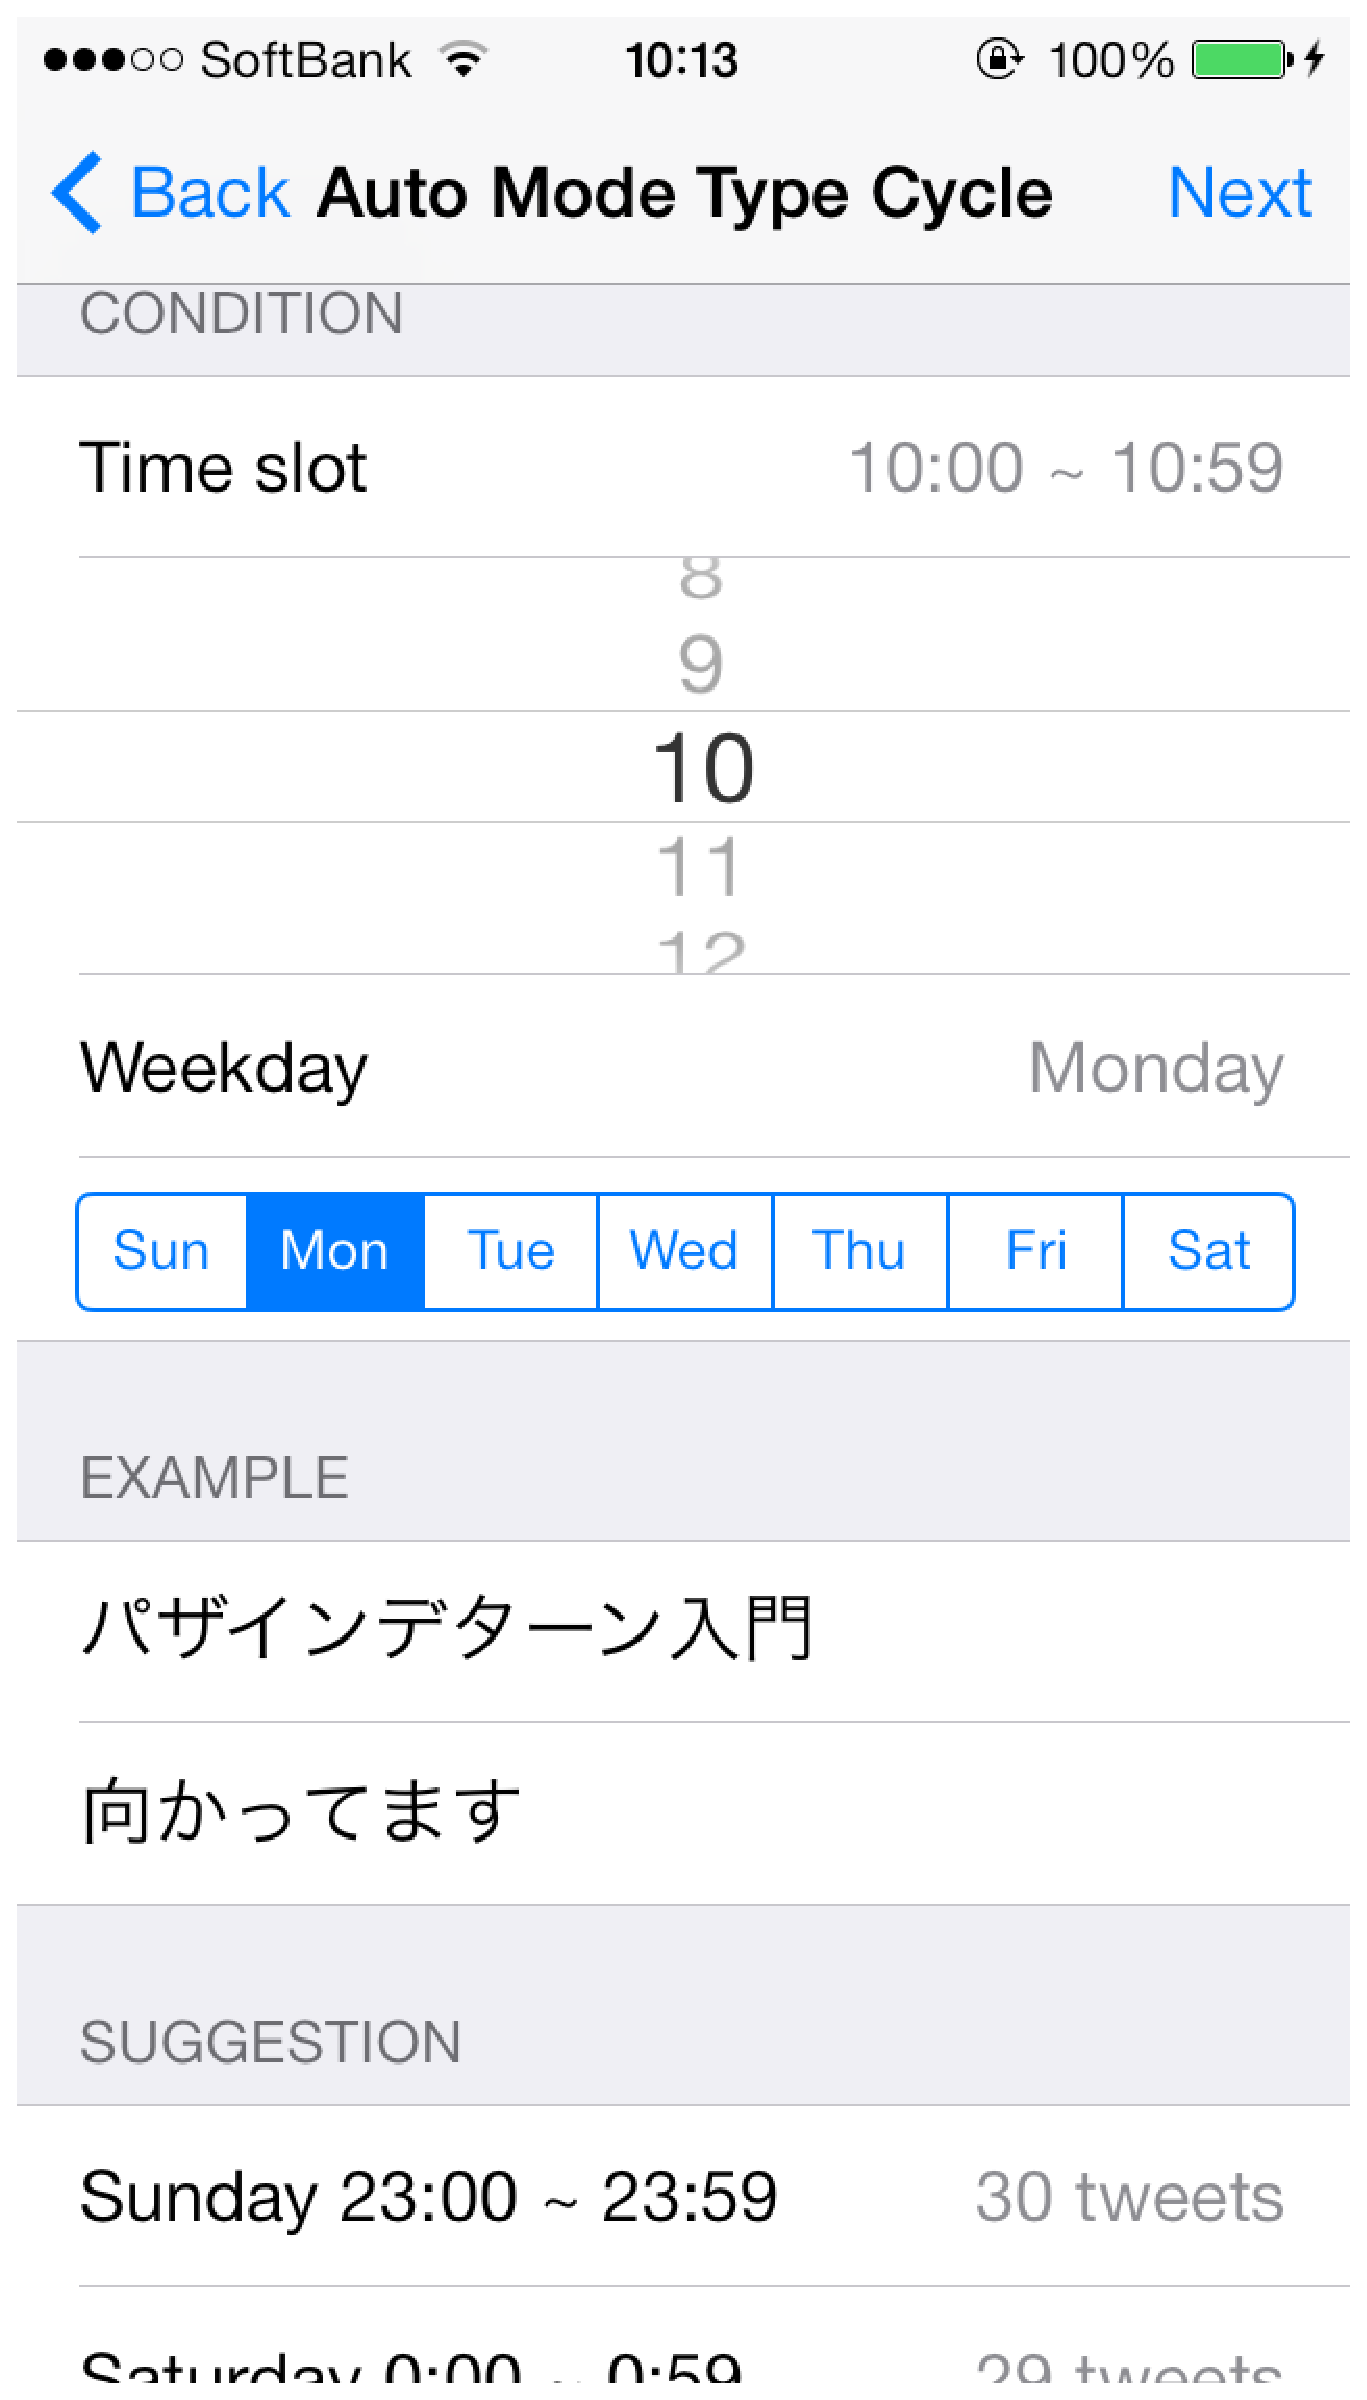
\includegraphics[width=60mm]{img/notifauthAutoCycle.eps}
  \end{center}
  \caption{Auto Mode Type Cycleの設定画面}
  \label{fig:notifauthAutoCycle}
\end{figure}

\subsubsection{具体例}
例えば,図\ref{fig:notifauthAutoCycle}に表示されているのと同じ,月曜日の10:00〜10:59に投稿されたツイートを秘密情報とするように設定すると,図\ref{fig:autoCycleSystem}のように,1/20時点で認証操作を行う際には,「今日はゼミだ」が秘密情報となるが,その2週間後である2/4に認証を行った時には「寝坊した!」も正しい秘密情報の一つとして追加され,「今日はゼミだ」と「寝坊した!」のどちらを選択しても認証は失敗する,という状況になる.

\subsection{Manual Mode}
この認証方式は,自分のツイート最新200件を取得し,その中から任意に1つ秘密情報となるものを選ぶ.
この方式では,認証時に新たなツイートの取得を行わないため,ダミーの選択肢は秘密情報を設定した時の群から選びぬかれる.

\subsubsection{意図}
当方式は3つの手法の中で最も単純であり,他の2つの方式のような特徴を持たない.
そのため,以下の欠点を抱えている.
\begin{itemize}
  \item 認証中の画面において,選択肢の中に必ず選択肢の一つとして表示されるため,総当たり攻撃や統計的手法を用いた攻撃に対して強度をもたない
\end{itemize}

\subsubsection{設定方法}
直近のツイートを最大200件取得し,これのうちどれを秘密情報とするかを図\ref{fig:notifauthManual}のように手動で選択し設定する.
ここで設定したツイートは,もう一度設定しない限りは実験終了まで固定されたままである.

\begin{figure}
  \begin{center}
    \includegraphics[width=60mm]{img/notifauthManual.eps}
  \end{center}
  \caption{Manual Modeの設定画面}
  \label{fig:notifauthManual}
\end{figure}

\section{認証操作}\label{sec:authentication}
第\ref{subsec:forMobile}節で述べたように,本システムでは認証操作にロック画面中の通知機能を利用し開発を行った.
実験を行いやすくするために本論文中の実装では,上記のロック画面を模した環境(図\ref{fig:notifauthTest})をアプリケーション内に実装した.

通知の表示画面を模した認証画面(図\ref{fig:notifauthTest}左)では,10個のツイートの本文と,当てはまるものがなかった場合に選択する「No match」の11つの候補を表示している.
その中から,正解だと思われるものを,指でタップし,そのまま右にスライドすることで,次の画面に遷移する.
なお,正解でないツイートの群をこれ以降,ダミーと呼ぶ.

PINの入力画面を模した認証画面(図\ref{fig:notifauthTest}右)では,0から9までのボタンと「キャンセル」ボタンが存在し,要求される桁数の入力が完了した段階で,結果画面に遷移する.
また,入力の途中で間違えた数字を選択してしまった場合は「キャンセル」ボタンをタップすることで,前画面に戻る.
その際,表示される候補の内容や順番は新たに更新される.

\begin{figure}[ht]
  \begin{center}
    \epsfig{file=img/notificationSliding.eps,scale=0.35}
  \end{center}
  \caption{ロック画面上における通知の選択(スライド)動作の例}
  \label{fig:notificationSliding}
\end{figure}

\begin{figure}[ht]
  \begin{minipage}{0.5\hsize}
    \begin{center}
      \includegraphics[width=60mm]{img/notifauthNotificationTest.eps}
    \end{center}
  \end{minipage}
  \begin{minipage}{0.5\hsize}
    \begin{center}
      \includegraphics[width=60mm]{img/notifauthPINTest.eps}
    \end{center}
  \end{minipage}
  \caption{左:ロック画面における通知の表示画面を模した認証画面,右:ロック画面におけるPINの入力画面を模した認証画面}
  \label{fig:notifauthTest}
\end{figure}

\section{システムの使用にあたって}
本システムを利用するための留意事項を表\ref{tbl:requirements}に記す.
本システムは,Apple社が開発した携帯端末向けオペレーティングシステムであるiOS 7を搭載している携帯端末を利用し,Twitterアカウントを保持していることが利用可能な最低条件となる.
加えて,1日あたりのツイートの数が極端に少ないと最低限度の安全性を保てない恐れが生じるため,定期的に複数のツイートを行っていることを推奨条件とした.
また,本アプリケーションは,OAuth\footnote{デスクトップ,モバイル,WebアプリケーションなどにセキュアなAPI認可の標準的手段を提供するためのオープンなプロトコル}を用いたTwitterとの連携を行わなければ利用することができない.

\begin{table}[htpb]
  \begin{center}
    \caption{留意事項}
    \label{tbl:requirements}
    \vspace{4mm}
    \begin{tabular}{ll}
    \bhline
    必要条件 & (1)iOS7を利用していること \\
     & (2)Twitterアカウントを保持していること \\
    推奨条件 & 定期的に複数のツイートを行っていること \\
    事前準備 & TwitterのOAuthを用いて本ソフトウェアと連携する \\
    \bhline
    \end{tabular}
  \end{center}
\end{table}

\section{開発環境}
本システムの開発環境を表\ref{tbl:environment}に示す.
本システムはApple社のパーソナルコンピュータ用OSであるMac OS Xと同社の総合開発環境であるXcodeを用いて開発を行った.
また,動作に必要なプラットフォームとして同社のiOSバージョン7.0以降を搭載している端末を要求し,サポート対象となっている現行機種の9割以上で動作の確認を行っている.
\begin{table}[htpb]
  \begin{center}
    \caption{開発環境}
    \label{tbl:environment}
    \vspace{4mm}
    \begin{tabular}{ll}
    \bhline
    プラットフォーム & Apple社 iOSバージョン7.0以上 \\
    開発言語 & Objective-C \\
    実装環境 & Mac OS X 10.9, Xcode5 \\
    動作確認環境 & iPhone 4,iPhone 4S,iPhone 5,iPhone 5S,iPod touch \\
    \bhline
    \end{tabular}
  \end{center}
\end{table}

\newpage
